\section*{Sistemas con \(N> 2\) grados de libertad}


\item
\begin{minipage}[t][1.8cm]{0.65\textwidth}
\textbf{Molécula triatómica}
Se esquematiza en la figura una molécula triatómica simétrica.
Entre dos átomos de masa $m$ hay uno de masa $M = 2 m$.
Se modelan los enlaces bajo el modelo de elasticidad de Hooke con constante $k$ y longitud natural $\ell_0$.
\end{minipage}
\begin{minipage}[c][0cm][t]{0.7\textwidth}
%   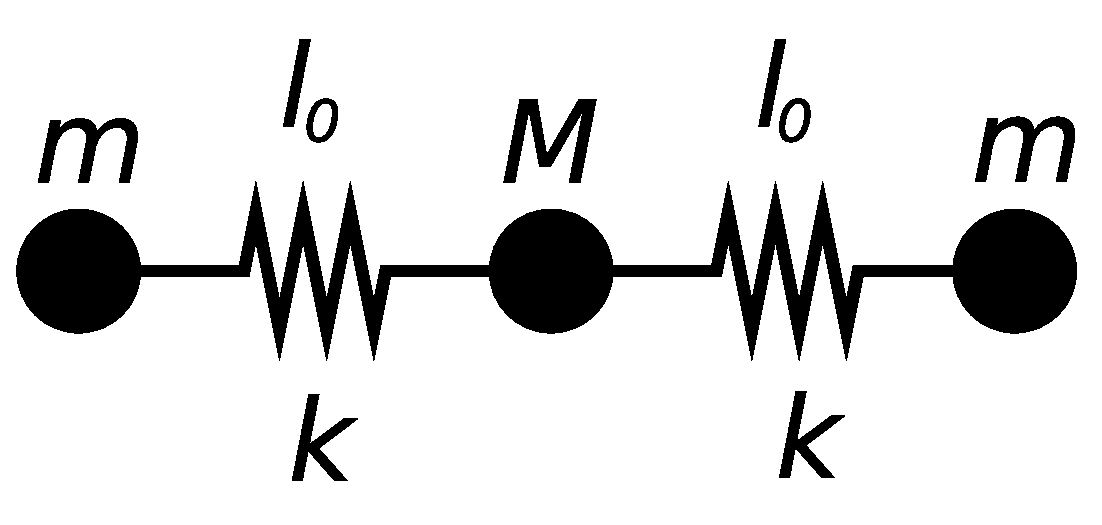
\includegraphics[width=\textwidth]{ej1-9}
	\begingroup
		% \tikzset{every picture/.style={scale=0.4}}%
		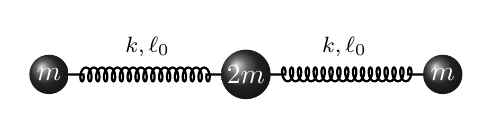
\begin{tikzpicture}
\coordinate (A) at (-2.5,0);
\coordinate (B) at (0,0);
\coordinate (C) at (2.5,0);

% \draw[very thick](-5,-1)--(-5,1);
% \draw[very thick](5,-1)--(5,1);

\draw[thick,decoration={coil,aspect=-.5,post length=0.35cm,segment length=1mm,pre length=0.5cm},decorate](B)--node[yshift=10]{\footnotesize $k, \ell_0$}(A);
\draw[thick,decoration={coil,aspect=-.5,post length=0.35cm,segment length=1mm,pre length=0.5cm},decorate](B)--node[yshift=10]{\footnotesize $k, \ell_0$}(C);
% \draw[thick,{Ellipse[open]}-](-5.125,0|-A)--(A);
% \draw[thick,{Ellipse[open]}-](5.125,0|-C)--(C);

% \foreach \x in {-2.5,0,2.5} \draw[dotted](\x,-1)--(\x,1);

\shade[ball color=black!80](A)circle(0.25)node[]{\color{white} $m$};
\shade[ball color=black!80](B)circle(0.315)node[]{\color{white} $2 m$};
\shade[ball color=black!80](C)circle(0.25)node[]{\color{white} $m$};

% \draw[{Stealth[]}-{Stealth[]}](-5,-0.75)--node[anchor=north]{$a$}(-2.5,-0.75);
% \draw[{Stealth[]}-{Stealth[]}](-2.5,-0.75)--node[anchor=north]{$a$}(0,-0.75);
% \draw[{Stealth[]}-{Stealth[]}](0,-0.75)--node[anchor=north]{$a$}(2.5,-0.75);
% \draw[{Stealth[]}-{Stealth[]}](2.5,-0.75)--node[anchor=north]{$a$}(5,-0.75);

\end{tikzpicture}
}
	\endgroup
\end{minipage}
\begin{enumerate}
	\item Encuentre las ecuaciones para la dinámica de cada átomo en la dirección longitudinal a la molécula, \(\hat{x}\).
	Asuma que los átomos tienen impedido un movimiento transversal.
	\item Halle las frecuencias de los modos normales. 
	\item Dibuje las configuraciones de cada modo. 
	\item Si el centro de masa de la molécula se mueve con $\vec{v}_0 = \mathrm{cte}\, \hat{x}$, escriba la solución $\vec{x}(t)$.
	\item Determine las condiciones iniciales para excitar sólo el modo de mayor frecuencia.
\end{enumerate}



\item
% \begin{minipage}[t][2.2cm]{0.5\textwidth}
Analice las oscilaciones transversales del problema anterior.
Para su mejor comprensión puede imaginarlo como el esquema de la figura, en el cual las partículas de los extremos pueden subir/bajar pero solidarios a la barra enhebrada a los vástagos laterales. 
% \end{minipage}
% \begin{minipage}[c][0cm][t]{0.45\textwidth}
%   \includegraphics[width=\textwidth]{\detokenize{moléculaT}}
% \end{minipage}
\begin{figure}[h]
	\centering
	\begin{tikzpicture}
\coordinate (A) at (-2.5,0);
\coordinate (B) at (0,0);
\coordinate (C) at (2.5,0);

\draw[very thick](-5,-1)--(-5,1);
\draw[very thick](5,-1)--(5,1);

\draw[thick,decoration={coil,aspect=-.5,post length=0.35cm,segment length=1mm,pre length=0.5cm},decorate](B)--node[yshift=10]{\footnotesize $k, \ell_0 < a$}(A);
\draw[thick,decoration={coil,aspect=-.5,post length=0.35cm,segment length=1mm,pre length=0.5cm},decorate](B)--node[yshift=10]{\footnotesize $k, \ell_0 < a$}(C);
\draw[thick,{Ellipse[open]}-](-5.125,0|-A)--(A);
\draw[thick,{Ellipse[open]}-](5.125,0|-C)--(C);

\foreach \x in {-2.5,0,2.5} \draw[dotted](\x,-1)--(\x,1);

\shade[ball color=black!80](A)circle(0.25)node[]{\color{white} $m$};
\shade[ball color=black!80](B)circle(0.315)node[]{\color{white} $2 m$};
\shade[ball color=black!80](C)circle(0.25)node[]{\color{white} $m$};

\draw[{Stealth[]}-{Stealth[]}](-5,-0.75)--node[anchor=north]{$a$}(-2.5,-0.75);
\draw[{Stealth[]}-{Stealth[]}](-2.5,-0.75)--node[anchor=north]{$a$}(0,-0.75);
\draw[{Stealth[]}-{Stealth[]}](0,-0.75)--node[anchor=north]{$a$}(2.5,-0.75);
\draw[{Stealth[]}-{Stealth[]}](2.5,-0.75)--node[anchor=north]{$a$}(5,-0.75);

\end{tikzpicture}

\end{figure} 
\begin{enumerate}
	\item Encuentre las ecuaciones de movimiento de las partículas.
	¿Qué diferencia hay en el caso con resortes \emph{slinky} y con $\ell_0 \neq 0$ en las ecuaciones de movimiento bajo la aproximación de pequeñas oscilaciones? 
	\item Halle las frecuencias de los modos normales.
	\item Dibuje la configuración correspondiente a cada modo normal.
Determine los desplazamientos de cada partícula como función del tiempo (solución más general posible para cada partícula).
	\item ¿Qué condiciones iniciales que permiten excitar sólo el segundo modo?
	\item Si se fuerza la partícula del centro con frecuencias incrementalmente mayores, ¿qué modos se van observando?
	\item ¿Cómo se modifican los resultados anteriores si la párticula en la derecha se enlaza, no un vástago sino, a una pared a través de un resorte igual a los demás como muestra la siguiente figura?
	\begin{figure}[h]
		\centering
		\begin{tikzpicture}
\coordinate (A) at (-2.5,0);
\coordinate (B) at (0,0);
\coordinate (C) at (2.5,0);

\draw[very thick](-5,-1)--(-5,1);
% \draw[very thick](5,-1)--(5,1); % pared derecha
\draw [very thick] (5,-1) coordinate (screen) -- (5,1); % pared derecha
\fill [pattern = north east lines] (screen) rectangle +(0.25,2); % pared derecha pattern

\draw[thick,decoration={coil,aspect=-.5,post length=0.35cm,segment length=1mm,pre length=0.5cm},decorate](B)--node[yshift=10]{\footnotesize $k,\ell_0 < a$}(A);
\draw[thick,decoration={coil,aspect=-.5,post length=0.35cm,segment length=1mm,pre length=0.5cm},decorate](B)--node[yshift=10]{\footnotesize $k,\ell_0 < a$}(C);
\draw[thick,{Ellipse[open]}-](-5.125,0|-A)--(A);
\draw[thick,decoration={coil,aspect=-.5,post length=0.35cm,segment length=1mm,pre length=0.2cm},decorate](5,0)--node[yshift=10]{\footnotesize $k,\ell_0 < a$}(C);

\foreach \x in {-2.5,0,2.5} \draw[dotted](\x,-1)--(\x,1);

\shade[ball color=black!80](A)circle(0.25)node[]{\color{white} $m$};
\shade[ball color=black!80](B)circle(0.315)node[]{\color{white} $2 m$};
\shade[ball color=black!80](C)circle(0.25)node[]{\color{white} $m$};

\draw[{Stealth[]}-{Stealth[]}](-5,-0.75)--node[anchor=north]{$a$}(-2.5,-0.75);
\draw[{Stealth[]}-{Stealth[]}](-2.5,-0.75)--node[anchor=north]{$a$}(0,-0.75);
\draw[{Stealth[]}-{Stealth[]}](0,-0.75)--node[anchor=north]{$a$}(2.5,-0.75);
\draw[{Stealth[]}-{Stealth[]}](2.5,-0.75)--node[anchor=north]{$a$}(5,-0.75);

\end{tikzpicture}

		% \includegraphics[clip,scale=0.5]{\detokenize{moléculaT_fijo_libre}}
	\end{figure} 
\end{enumerate}



\item
\begin{minipage}[t][1.2cm]{0.6\textwidth}
Considere el sistema de la figura, en la que los resortes verticales tienen longitud natural $l_0$ y constante $k_1$, y los horizontales $a_0= 0$ (son ``slinkies'') y $k_2$.
Calcule las frecuencias propias y los modos normales. 
\end{minipage}
\begin{minipage}[c][1.2cm][t]{0.35\textwidth}
  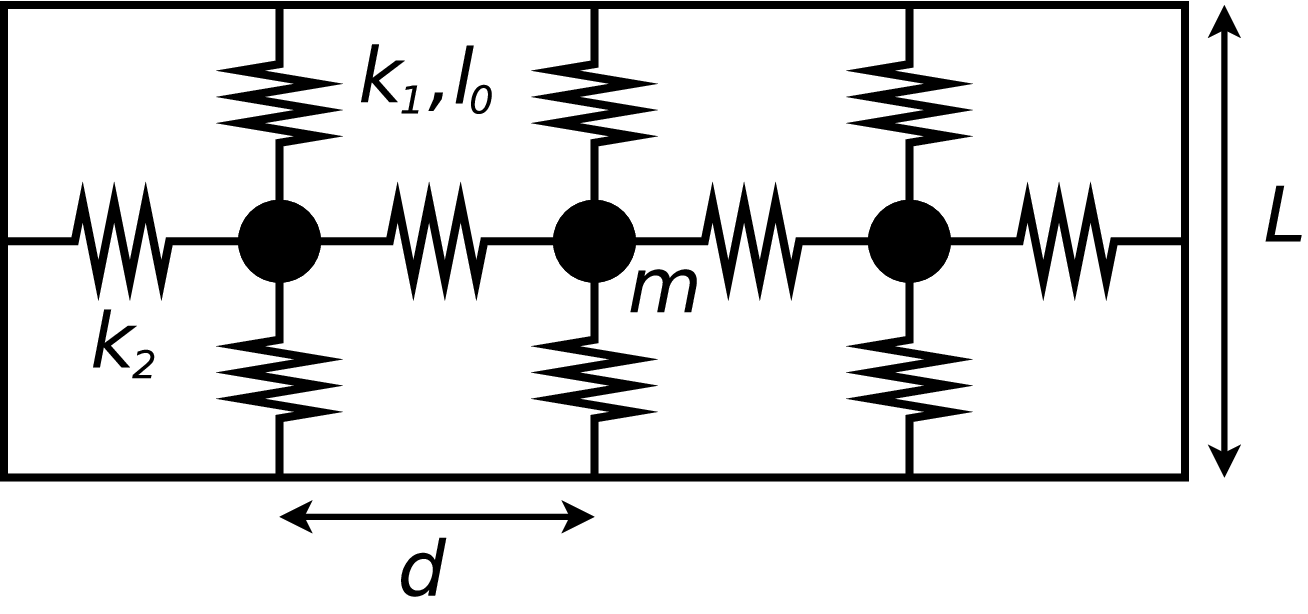
\includegraphics[width=\textwidth]{ej1-10}
\end{minipage}
